\documentclass[11pt]{article}
\usepackage{homework}
\usepackage{slashed}
\usepackage{simpler-wick}

\classname{443}
\homeworknum{5}



\begin{document}

% Environments

\newcommand{\state}[2]{\begin{statement}{#1} #2 \end{statement}}
\newcommand{\prob}[2]{\begin{problem}{#1} #2 \end{problem}}
\newcommand{\subprob}[1]{\begin{subproblem} #1 \end{subproblem}}
\newcommand{\sol}[1]{\begin{solution} #1 \end{solution}}
\newcommand{\fig}[2]{\begin{figure} \centering #2  \label{#1} \end{figure}}

\newcommand{\makebib}{
	\vfill
	\color{black}
	\nocite{*}
	\bibliography{references}{}
	\bibliographystyle{lucas_unsrt}
}
	

% Implication

\newcommand{\qwhere}{\quad \text{where} \quad}
\newcommand{\qimplies}{\quad \implies \quad}
\newcommand{\impliesq}{\implies \quad}



% Brackets

\newcommand{\paren}[1]{\left( #1 \right)}
\newcommand{\brac}[1]{\left[ #1 \right]}
\newcommand{\curly}[1]{\left\{ #1 \right\}}


% Greek

\newcommand{\alp}{\alpha}
\newcommand{\bet}{\beta}
\newcommand{\gam}{\gamma}
\newcommand{\del}{\delta}
\newcommand{\eps}{\epsilon}
\newcommand{\zet}{\zeta}
\newcommand{\tht}{\theta}
\newcommand{\kap}{\kappa}
\newcommand{\lam}{\lambda}
\newcommand{\sig}{\sigma}
\newcommand{\ups}{\upsilon}
\newcommand{\omg}{\omega}

\newcommand{\Gam}{\Gamma}
\newcommand{\Del}{\Delta}
\newcommand{\Tht}{\Theta}
\newcommand{\Lam}{\Lambda}
\newcommand{\Sig}{\Sigma}
\newcommand{\Omg}{\Omega}


% Text

\newcommand{\where}{\text{where }}

% Problem 1

\newcommand{\Hint}{H_\text{int}}
\newcommand{\ddcx}{\dd[3]{x}}
\newcommand{\psib}{\bar{\psi}}

\newcommand{\mh}{m_h}
\newcommand{\mmu}{m_\mu}
\newcommand{\me}{m_e}
\newcommand{\ma}{m_a}

\newcommand{\aexpt}{a_\text{expt.}}
\newcommand{\aQED}{a_\text{QED}}
\renewcommand{\GeV}{\giga\electronvolt}

\newcommand{\gamt}{\gam^5}

\state{Spin-wave theory~(P\&S 11.1)}{\hfix}

\prob{ \label{1a}
	Prove the following wonderful formula: Let $\phix$ be a free scalar field with propagator $\ev{T \phix \phio} = \Dx$.  Then
	\eqn{show1}{
		\ev{ T e^{i \phix} e^{-i \phio} } = e^{[ \Dx - \Do ]}.
	}
	(The  factor $\Do$ gives a formally divergent adjustment of the overall normalization.)
}

\sol{
	According to P\&S~(9.18),
	\eq{
		\ev*{T \phi(\xq) \phi(\xw)}{\Omg} = \frac{\int \DDphi \phi(\xq) \phi(\xw) \exp[ i \int \ddqx \cL ]}{\int \DDphi \exp[ i \int \ddqx \cL ]}.
	}
	We use this expression to write the left-hand side of Eq.~\refeq{show1}:
	\eqn{thing1}{
		\ev{ T e^{i \phix} e^{-i \phio} } = \frac{\int \DDphi e^{i \phix} e^{-i \phio} \exp[ i \int \ddqy \cL ]}{\int \DDphi \exp[ i \int \ddqy \cL ]}
		= \frac{\int \DDphi \exp[i \phix - i \phio + i \int \ddqy \cL ]}{\int \DDphi \exp[ i \int \ddqy \cL ]}.
	}
	For a free Klein-Gordon~(i.e., scalar) field, Eq.~(9.39) tells us that the generating functional $\ZJ$ is given by
	\eq{
		\ZJ = \Zo \exp[ -\frac{1}{2} \int \ddqx \ddqy \Jx \DF(x - y) \Jy ],
	}
	where $\Zo = Z[0]$.  Thus, we want to find some $\Jy$ such that
	\eqn{thing1b}{
		\ev{ T e^{i \phix} e^{-i \phio} } = \frac{\ZJ}{\Zo}
	}
	where in general
	\eq{
		\ZJ = \int \DDphi \exp[ i \int \ddqx [ \cL + \Jx \phi(x) ] ]
	}
	by (9.34).  Inspecting Eq.~\refeq{thing1}, we recognize the denominator as $\Zo$ and see that if
	\eq{
		\Jy = \delq(y - x) - \delq(y)
	}
	we have an expression like Eq.~\refeq{thing1b}.  Collecting these findings, we have
	\al{
		\ans{ \ev{ T e^{i \phix} e^{-i \phio} } }&= \frac{\ZJ}{\Zo} \\
		&= \exp[ -\frac{1}{2} \int \ddqy \ddqz \Jy \DF(y - z) \Jz ] \\
		&= \exp[ -\frac{1}{2} \int \ddqy \ddqz \Jy \DF(y - z) [ \delq(z - x) - \delq(z) ] ] \\
		&= \exp[ -\frac{1}{2} \int \ddqy [ \delq(y - x) - \delq(y) ] [ \DF(y - x) - \DF(y) ] ] \\
		&= \exp[ -\frac{1}{2} [ \DF(0) - \DF(x) - \DF(-x) + \DF(0) ] ] \\
		&= \exp[ \DF(x) - \DF(0) ] \\
		&\ans{\; = e^{[ \Dx - \Do ]}, }
	}
	as we wanted to show. \qed
}



\prob{ \label{1b}
	We can use this formula in Euclidean field theory to discuss correlation functions in a theory with spontaneously broken symmetry for $T < \TC$.  Let us consider only the simplest case of a broken $O(2)$ or $U(1)$ symmetry.  We can write the local spin density as a complex variable
	\eq{
		\sx = \sqx + i \swx.
	}
	The global symmetry is the transformation
	\eq{
		\sx \to e^{-i \alp} \sx.
	}
	If we assume that the physics freezes the modulus of $\sx$, we can parameterize
	\eqn{sx}{
		\sx = A e^{i \phix}
	}
	and write an effective Lagrangian for the field $\phix$.  The symmetry of the theory becomes the translation symmetry
	\eqn{symmetry}{
		\phix \to \phix - \alp.
	}
	Show that (for $d > 0$) the most general renormalizable Lagrangian consistent with this symmetry is the free field theory
	\eqn{show1b}{
		\cL = \frac{1}{2} \rho(\vgrad \phi)^2.
	}
	In statistical mechanics, the constant $\rho$ is called the \emph{spin wave modulus}.  A reasonable hypothesis for $\rho$ is that it is finite for $T < \TC$ and tends to 0 as $T \to \TC$ from below.
}

\sol{
	In accordance with the Klein-Gordon Lagrangian in P\&S~(2.6),
	\eqn{KGL}{
		\cL_\text{K-G} = \frac{1}{2} (\pt \phi)^2 - \frac{1}{2} m^2 \phi^2,
	}
	we interpret $(\vgrad \phi)^2$ as $(\pt \phi)^2$.
	
	The Lagrangian cannot have terms of $\order{\phi^n}$ for any $n \neq 0$ since $\phi(x)$ is not invariant under Eq.~\refeq{symmetry}.  Any combination of derivatives of $\phi$ is invariant, however, since $\alp$ is a constant and does not contribute to any derivative.  Thus, only terms like $\pt^n \phi^m$ (where $n$ denotes a power of $\pt$) for $n, m > 0$ and $n \geq m$ are consistent with the symmetry of Eq.~\refeq{symmetry} for $d$ an integer.
	
	Now we must determine which of these terms are renormalizable.  We know that the Lagrangian must have dimension $d$, and that $\phi$ has dimension $(d - 2) / 2$.  Taking a derivative adds a mass dimension.  The theory is renormalizable if the coupling constant $\rho$ has dimension greater than or equal to 0~\cite[p.~322]{Peskin}.  Let $p$ be the dimension of $\rho$.  The dimension of our allowed term is then
	\eq{
		[ \rho \pt^n \phi^m ] = p + n + m \frac{d - 2}{2},
	}
	which we require to be equal to $d$.  Thus we seek solutions to the system of equations
	\al{
		d &= p + n + m \frac{d - 2}{2}, &
		n &\geq m, &
		p &\geq 0.
	}
	Solving with Mathematica, we find that this system has two solutions: $n = m = 2$ and $p = 0$; and $n = m = 1$ and $p = d / 2$.  However, the term $\pt \phi$ for $n = m = 1$ does not contribute to the action because it is a total derivative and does not contribute when the integral over $\cL$ is evaluated:
	\eq{
		\int \dd[d]{x} \pt\phi = \phi \bigg|_{-\infty}^\infty
		= 0.
	}
	Thus the only possibility is $n = m = 2$.  Note that
	\eq{
		\pt^2 \phi^2 = \pt(\pt \phi^2)
		= 2 \pt( \phi \pt \phi)
		= \pt \phi \pt \phi + \phi \pt^2 \phi
		= (\pt \phi)^2,
	}
	since $\phi \pt^2 \phi$ is not invariant under Eq.~\refeq{sx}.  This means that $\rho$ must be dimensionless and that the only allowed terms in the Lagrangian are proportional to $(\pt \phi)^2$, which is consistent with Eq.~\refeq{show1b}. \qed
}



\prob{
	Compute the correlation function $\ev{ \sx \sao }$.  Adjust $A$ to give a physically sensible normalization (assuming that the system has a physical cutoff at the scale of one atomic spacing) and display the dependence of this correlation function on $x$ for $d = 1, 2, 3, 4$.  Explain the significance of your results.
}

\sol{
	Applying Eq.~\refeq{sx},
	\eq{
		\ev{ \sx \sao } = \ev*{ A e^{i \phix} \As e^{-i \phio} }
		= \ev*{ \abs{A}^2 } \ev*{ e^{i \phix} e^{-i \phio} }.
	}
	Now we can apply Eq.~\refeq{show1} to find
	\eqn{thing1c}{
		\ans{ \ev{ \sx \sao } = \abs{A}^2 \exp[ D(x) - D(0) ], }
	}
	where $D(x - y)$ is a Green's function.  Since our Lagrangian is similar to the Klein-Gordon Lagrangian Eq.~\refeq{2.6}, our Green's function is similar to that of the Klein-Gordon operator, which is given by P\&S~(2.56):
	\eq{
		(\pt^2 + m^2) D(x - y) = -i \delq(x - y).
	}
	The Feynman prescription for this Green's function is given by (2.59),
	\eqn{DF}{
		\DF(x - y) = \int \ddqpf \frac{i}{p^2 - m^2 + i \eps} e^{-i p \cdot (x - y)}.
	}
	For the Lagrangian in Eq.~\refeq{show1b}, we set $m = 0$ and insert a factor of $\rho$:
	\eq{
		\rho \pt^2 D(x - y) = -i \deld(x - y),
	}
	so adapting Eq.~\refeq{DF} for this situation yields
	\eqn{DF}{
		\DF(x - y) = \frac{1}{\rho} \int \dddpf \frac{i}{p^2 + i \eps} e^{-i p \cdot (x - y)}.
	}
	We see that $\DF(0)$ diverges, so we absorb it into the constant to make the normalization physically sensible.  We can do this because, as we showed in \ref{1b}, the theory is renormalizable.  Define $A'$ such that
	\eq{
		{A'}^2 = \abs{A}^2 e^{-D(0)}.
	}
	Then Eq.~\refeq{thing1c} can be written
	\eq{
		\ans{ \ev{ \sx \sao } =  {A'}^2 e^{D(x)}. }
	}
	
	To evaluate the divergent integral $D(x)$, we look to the Feynman parameter method we have been using to solve divergent integrals.  Apparently, the Schwinger parametrization is useful in deriving the Feynman parametrization, and it is given by~\cite{Feynman}
	\eq{
		\frac{1}{A} = \intoi \dds e^{-s A}.
	}
	Using this equation, we can write Eq.~\refeq{DF} as
	\eq{
		\DF(x) = \frac{1}{\rho} \int \dddpf \frac{i}{p^2} e^{-i p \cdot x}
		= \frac{i}{\rho} \int \dddpf \intoi \dds e^{-s p^2} e^{-i p \cdot x}.
	}
	Now we can complete the square in the exponential to get a Gaussian integral:
	\al{
		\DF(x) &= \frac{i}{\rho} \int \dddpf \intoi \dds \exp[ -s p^2 - i p \cdot x + \frac{x^2}{4 s} - \frac{x^2}{4 s} ] \\
		&= \frac{i}{\rho} \int \dddpf \intoi \dds \exp[ -s \paren{ p + \frac{i x}{2 s} }^2 - \frac{x^2}{4 s} ] \\
		&= \frac{i}{\rho (2 \pi)^d} \intoi \dds e^{-x^2 / 4 s} \int \dd[d]{u} e^{-s u^2} \\
		&= \frac{i}{\rho (2 \pi)^{d}} \intoi \dds e^{-x^2 / 4 s} \sqrt{ \frac{(2\pi)^d}{(2s)^d} } \\
		&= \frac{i}{\rho (4 \pi)^{d / 2}} \intoi \dds \frac{e^{-x^2 / 4 s}}{s^{d / 2}}
	}
	where we have used~\cite{QFT}
	\eq{
		\int \exp( -\frac{1}{2} x \cdot A \cdot x ) \dd[n]{x} = \sqrt{\frac{(2\pi)^n}{\det A}},
	}
	with $A$ a $d \times d$ diagonal matrix $2s$.  Using Mathematica to integrate with respect to $s$, we find
	\eq{
		\DF(x) = \frac{i}{\rho (4 \pi)^{d / 2}} \frac{2^{d - 2}}{x^{d - 2}} \Gam(d / 2 - 1)
		= \frac{i}{4 \pi^d \rho} \Gam(d / 2 - 1) x^{2 - d}.
	}
	The gamma function diverges as $d \to 2$, so as we have done in previous problems, we expand about $\eps = 2 - d$.  Evaluating the series expansion using Mathematica, we obtain
	\eq{
		\DF(x) = \frac{i}{4 \pi^{1 - \eps} \rho} \Gam(\eps / 2) x^\eps
		\approx \frac{i}{4 \pi \rho} \paren{ \frac{2}{\eps} - \gam + 2 \ln(\pi x) }
		\sim \frac{i}{2 \pi \rho} \ln(x)
		= i \ln(\frac{1}{x^{2 \pi \rho}}).
	}
	We Wick rotate $x \to i x$.  Then the dependence of the correlation function on $x$ for $d = 1, 2, 3, 4$ is
	\ans{\al{
		(d = 1) &\qquad \ev{ \sx \sao } \sim e^{-x / 2 \sqrt{\pi} \rho}, &
		(d = 2) &\qquad \ev{ \sx \sao } \sim x^{2 \pi \rho}, \\
		(d = 3) &\qquad \ev{ \sx \sao } \sim \frac{1}{x}, &
		(d = 4) &\qquad \ev{ \sx \sao } \sim \frac{1}{x^2}.
	}}%
	In $d > 2$ dimensions, the expectation value of the correlation function tends to 0 at large distances $x$.  For $d > 2$, it drops off more quickly as $d$ increases.  The $d \leq 2$ cases depend on $\rho$, which we assume is positive.  The $d = 1$ case drops off with increasing distance, and more quickly with smaller $\rho$.  For $d = 2$, the expectation value of the correlation function increases with increasing distance, and it blows up more quickly with larger $\rho$.
	
	These results are consistent with the Mermin--Wagner theorem, which states that a continuous symmetry cannot be broken in $d \leq 2$ dimensions~\cite{CMW}.  That is, in $d \leq 2$ dimensions, a symmetry-breaking field cannot have a nonzero vacuum expectation value~\cite[p.~460]{Peskin}.  A physical explanation is that each spin has more nearest neighbors in higher dimensions.  Since the spins are inclined to align with their neighbors, there is a higher degree of correlation in higher dimensions at the same distance.  In two dimensions, the correlations are weak enough that they are overpowered by the field fluctuations.
}


\state{Bhabha scattering (Peskin \& Schroeder 5.2)}{
	Compute the differential cross section $\dv*{\sig}{(\cos\tht)}$ for Bhabha scattering, $\elp \elm \to \elp \elm$.  You may work in the limit $\Ecm \gg \me$, in which it is permissible to ignore the electron mass.  There are two Feynman diagrams; these must be added in the invariant matrix element before squaring.  Be sure that you have the correct relative sign between these diagrams.  The intermediate steps are complicated, but the final result is quite simple.  In particular, you may find it useful to introduce the Mandelstam variables $s$, $t$, and $u$.  Note that, if we ignore the electron mass, $s + t + u = 0$.  You should be able to cast the differential cross section into the form
	\eq{
		\dv{\sig}{(\cos\tht)} = \frac{\pi \alp^2}{s} \brac{ u^2 \paren{ \frac{1}{s} + \frac{1}{t} }^2 + \paren{ \frac{t}{s} }^2 + \paren{ \frac{s}{t} }^2 }.
	}
	Rewrite this formula in terms of $\cos\tht$ and graph it.  What feature of the diagrams causes the differential cross section to diverge as $\tht \to 0$?
}

\sol{
	The two Feynman diagrams are the $s$- and $t$-channel diagrams~\cite[p.~157]{Peskin}.  \hl{Draw them.}  
	
	The interaction Hamiltonian for QED is Peskin \& Schroeder~(4.129),
	\eq{
		\Hint = \int \ddcx e \psib \gamm \psi \Asm,
	}
	so the interaction is $\psib \Asm \gamm \psi$~\cite[p.~226]{Schwartz}.  Now we can write the matrix element for the interaction:
	\eq{
		\mel*{\vp, \vkk}{(\psib \Asm \gamm \psi)_x (\psib \Asm \gamm \psi)_y}{\vp', \vkk'}.
	}
	By Peskin \& Schroeder~(4.118),
	\al{
		\ket*{\vp, \vkk} &\sim \apdag \akdag \ket{0}, &
		\bra*{\vp', \vkk'} &\sim \bra{0} \akp \app.
	}
	Then the contractions for the $s$-channel diagram are
	\eq{
		\ev*{\wick{\c2{\akp} \c1{\app} (\c1{\psib} \Asm \gamm \c2{\psi})_x} \wick{(\c2{\psib} \Asm \gamm \c1{\psi})_y \c1{\apdag} \c2{\akdag}}}{0}.
	}
	For the $t$ channel,
	\al{
		\ev*{\wick{\c2{\akp} \c1{\app} (\c4{\psib} \Asm \gamm \c2{\psi})_x (\c1{\psib} \Asm \gamm \c3{\psi})_y \c3{\apdag} \c4{\akdag}}}{0}
		&= -\ev*{\wick{\c2{\akp} \c1{\app} (\Asm \gamm \c2{\psi} \c4{\psib})_x (\c1{\psib} \Asm \gamm \c3{\psi})_y \c3{\apdag} \c4{\akdag}}}{0} \\
		&= \ev*{\wick{\c2{\akp} \c1{\app} (\Asm \gamm \c2{\psi})_x \c1{\psib}_y} \wick{\c2{\psib}_x (\Asm \gamm \c1{\psi})_y \c1{\apdag} \c2{\akdag}}}{0} \\
		&= - \ev*{\wick{\c2{\akp} \c1{\app} \c1{\psib}_y (\Asm \gamm \c2{\psi}} \wick{\c2{\psib})_x (\Asm \gamm \c1{\psi})_y \c1{\apdag} \c2{\akdag}}}{0}.
	}
	We needed to swap the order of adjacent fields three times, which gives an overall minus sign~\cite[p.~118]{Peskin}.  This means we subtract the $t$ channel diagram: \hl{subtract them}
	
	The matrix element for the $s$ channel is the same as Peskin \& Schroeder~(5.1),
	\eq{
		i \cM = \frac{i e^2}{s} \vbk \gamm \up \ubpp \gamsm \vkp.
	}
	For the $t$ channel, it is~\cite[p.~153]{Peskin}
	\eq{
		i \cM = \frac{i e^2}{t} \ubpp \gamm \up \vbk \gamsm \vkp
	}
	where we have used the Mandelstam variables~\hl[cite].  Their difference is
	\eq{
		i \cM = i e^2 \brac{ \frac{\vbk \gamm \up \ubpp \gamsm \vkp}{s} - \frac{\ubpp \gamm \up \vbk \gamsm \vkp}{t} },
	}
	which means~\cite[p.~132]{Peskin}
	\eq{
		-i \cMs = -i e^2 \brac{ \frac{\ubp \gamm \vk \vbkp \gamsm \upp}{s} - \frac{\ubp \gamm \upp \vbkp \gamsm \vk}{t} }.
	}
	Then
	\al{
		\abs{\cM}^2 &= e^4 \left[ \frac{\vbk \gamm \up \ubpp \gamsm \vkp \ubp \gamn \vk \vbkp \gamsn \upp}{s^2} - \frac{\vbk \gamm \up \ubpp \gamsm \vkp \ubp \gamn \upp \vbkp \gamsn \vk}{s t} \right. \\
		&\hspace{1.5em} \left. \phantom{=\ } - \frac{\ubpp \gamm \up \vbk \gamsm \vkp \ubp \gamn \vk \vbkp \gamsn \upp}{s t} + \frac{\ubpp \gamm \up \vbk \gamsm \vkp \ubp \gamn \upp \vbkp \gamsn \vk}{t^2} \right].
	}
	Note that~\cite[p.~132, 153]{Peskin}
	\al{
		\sumspins \vbk \gamm \up \ubpp \gamsm \vkp \ubp \gamn \vk \vbkp \gamsn \upp &= \Tr( \ksl \gamm \psl \gamn ) \Tr( \psl' \gamsm \ksl' \gamsn ), \\
		\sumspins \ubpp \gamm \up \vbk \gamsm \vkp \ubp \gamn \upp \vbkp \gamsn \vk &= \Tr( \psl' \gamm \psl \gamn ) \Tr( \ksl \gamsm \ksl' \gamsn ),
	}
	where we have taken $m \to 0$.  Writing the other two using components,
	\al{
		\sumspins \brac{ \vbk \gamm \up \ubpp \gamsm \vkp \ubp \gamn \upp \vbkp \gamsn \vk + \cc }
		&= \sumssp \sumrrp \brac{ \vbsar \gammsab \usbs \ubscspp \gamsmcd \vsdrp \ubses \gamnef \usfsp \vsgrp \gamsngh \vshr + \cc } \\
		&= \sumssp \sumrrp \brac{ \vshr \vbsar \gammsab \usbs \ubses \gamnef \usfsp \ubscspp \gamsmcd \vsdrp \vsgrp \gamsngh + \cc} \\
		&= \ksl_{h a} \gammsab \psl_{b e} \gamnef \psl'_{f c} \gamsmcd \ksl'_{d g} \gamsngh + \cc \\
		&= \Tr( \ksl \gamm \psl \gamn \psl' \gamsm \ksl' \gamsn ) + \cc
	}
	where we have used Peskin \& Schroeder~(5.3),
	\al{
		\sums \usp \ubsp &= \psl + m, &
		\sums \vsp \vbsp &= \psl - m,
	}
	and $m = 0$.  This gives us the matrix element
	\eq{
		\abs{\cM}^2 = e^4 \paren{ \frac{\Tr( \ksl \gamm \psl \gamn ) \Tr( \psl' \gamsm \ksl' \gamsn )}{s^2} - \frac{\Tr( \ksl \gamm \psl \gamn \psl' \gamsm \ksl' \gamsn ) + \cc}{s t} + \frac{\Tr( \psl' \gamm \psl \gamn ) \Tr( \ksl \gamsm \ksl' \gamsn )}{t^2} }.
	}
	We need to average over spins: $\sumspins \abs{\cM}^2 / 4$~\cite[p.~132]{Peskin}.  From (5.70) and (5.71),
	\al{
		\frac{1}{4} \sumspins \frac{e^4}{s^2} \Tr( \ksl \gamm \psl \gamn ) \Tr( \psl' \gamsm \ksl' \gamsn ) &= \frac{8 e^4}{s^2} \brac{ \paren{ \frac{t}{2} }^2 + \paren{ \frac{u}{2} }^2 }, \\
		\frac{1}{4} \sumspins \frac{e^4}{t^2} \Tr( \psl' \gamm \psl \gamn ) \Tr( \ksl \gamsm \ksl' \gamsn ) &= \frac{8 e^4}{t^2} \brac{ \paren{ \frac{s}{2} }^2 + \paren{ \frac{u}{2} }^2 }.
	}
	For the remaining terms, we adapt Peskin \& Schroeder~(5.69),
	\al{
		s &= (p + k)^2
		= (p' + k')^2, &
		t &= (p' - p)^2
		= (k' - k)^2, &
		u &= (k' - p)^2
		= (p' - k)^2.
	}
	For the $s$ channel in the massless limit~\cite[p.~156]{Peskin},
	\al{
		t &= -2 p \cdot p'
		= -2 k \cdot k', &
		u&= -2 p \cdot k'
		= -2 k \cdot p'.
	}
	Note that
	\al{
		\Tr( \ksl \gamm \psl \gamn \psl' \gamsm \ksl' \gamsn ) &= \ksa \psb \psr' \kss' \Tr( \gama \gamm \gamb \gamn \gamr \gamsm \gams \gamsn ) \\
		&= -2 \ksa \psb \psr' \kss' \Tr( \gama \gamr \gamn \gamb \gams \gamsn ) \\
		&= -8 \ksa \psb \psr' \kss' \Tr( \gama \gamr \gbs ) \\
		&= -8 \ksa \psb \psr' \kpb \Tr( \gama \gamr ) \\
		&= -32 \ksa \psb \psr' \kpb \gar \\
		&= -32 \ksa \ppa \psb \kpb \\
		&= -32 (k \cdot p') (p \cdot k') \\
		&= -8 u^2,
	}
	where we have used Peskin \& Schroeder~(5.9),
	\al{
		\gamm \gamn \gamr \gamsm &= 4 \gnr, &
		\gamm \gamn \gamr \gams \gamsm &= -2 \gams \gamr \gamn,
	}
	and (5.5), $\Tr(\gamm \gamn) = 4 \gmn$.  Then the matrix element is
	\aln{
		\frac{1}{4} \sumspins \abs{\cM^2} &= \frac{8 e^4}{s^2} \brac{ \paren{ \frac{t}{2} }^2 + \paren{ \frac{u}{2} }^2 } + \frac{4 e^4}{s t} u^2 + \frac{8 e^4}{t^2} \brac{ \paren{ \frac{s}{2} }^2 + \paren{ \frac{u}{2} }^2 } \notag \\
		&= 2 e^4 \brac{ \paren{ \frac{t}{s} }^2 + \frac{u^2}{s^2} + 2 \frac{u^2}{s t} + \paren{ \frac{s}{t} }^2 + \frac{u^2}{t^2} } \notag \\
		&= 2 e^4 \brac{ u^2 \paren{ \frac{1}{s^2} + 2 \frac{1}{s t} + \frac{1}{t^2} } + \paren{ \frac{t}{s} }^2 + \paren{ \frac{s}{t} }^2 } \notag \\
		&= 32 \pi^2 \alp^2 \brac{ u^2 \paren{ \frac{1}{s} + \frac{1}{t} }^2 + \paren{ \frac{t}{s} }^2 + \paren{ \frac{s}{t} }^2 }. \label{ans2a}
	}
	By Peskin \& Schroeder~(4.85), the differential cross section for four particles of the same mass is
	\eq{
		\dv{\sig}{\Omg} = \frac{\abs{\cM}^2}{64 \pi^2 \Ecm^2}.
	}
	In the center-of-mass frame, $\Ecm = (p + k) = \sqrt{s}$.  Feeding in Eq.~\refeq{ans2a},
	\eq{
		\dv{\sig}{\Omg} = \frac{1}{64 \pi^2 \Ecm^2} \frac{1}{4} \sumspins \abs{\cM^2}
		= \frac{\alp^2}{2 s} \brac{ u^2 \paren{ \frac{1}{s} + \frac{1}{t} }^2 + \paren{ \frac{t}{s} }^2 + \paren{ \frac{s}{t} }^2 }.
	}
	Noting that $\ddOmg = \ddcost \ddphi$ and $\int \ddphi = 2\pi$, we integrate over $\phi$ to find
	\eqn{ans2b}{
		\ans{ \dv{\sig}{(\cos\tht)} = \frac{\pi \alp^2}{s} \brac{ u^2 \paren{ \frac{1}{s} + \frac{1}{t} }^2 + \paren{ \frac{t}{s} }^2 + \paren{ \frac{s}{t} }^2 } }
	}
	as desired. \qed
	
	From Peskin \& Schroeder~(5.72),
	\al{
		s &= \Ecm^2, &
		t &= -2 \abs{\vp}^2 (1 - \cos\tht), &
		u &= -2 \abs{\vp}^2 (1 + \cos\tht).
	}
	Feeding these into Eq.~\refeq{ans2b},
	\aln{
		\dv{\sig}{(\cos\tht)} &= \frac{\pi \alp^2}{\Ecm^2} \brac{ 4 \abs{\vp}^4 (1 + \cos\tht)^2 \paren{ \frac{1}{\Ecm^2} - \frac{1}{2 \abs{\vp}^2 (1 - \cos\tht)} }^2 + \paren{ -\frac{2 \abs{\vp}^2 (1 - \cos\tht)}{\Ecm^2} }^2 + \paren{ -\frac{\Ecm^2}{2 \abs{\vp}^2 (1 - \cos\tht)} }^2 } \notag \\
		&= \ans{ \frac{4 \pi \alp^2 \abs{\vp}^4}{\Ecm^2} \brac{ \paren{ \frac{(1 + \cos\tht)^4}{\Ecm^2} - \frac{(1 + \cos\tht)^4}{2 \abs{\vp}^2 (1 - \cos\tht)} }^2 + \paren{ \frac{1 - \cos\tht}{\Ecm^2} }^2 + \paren{ \frac{\Ecm^2}{1 - \cos\tht} }^2 }. } \label{ans2}
	}
	A graph is shown in Fig.~\ref{f2}.  The differential cross section diverges as $\tht \to 0$ since the photon in the diagrams is nearly on shell; that is, $q^2 \to 0$~\cite[p.~155]{Peskin}.  When the mediating photon is massless~(on shell), electrons that are separated by an infinite distance can still scatter off each other.  Since they are so far apart, however, the angle of scattering approaches 0.  Since any electron anywhere in the universe may be scattering off another given electron with $\tht \approx 0$, the scattering cross section must blow up there.
	
	\begin{figure} \centering
		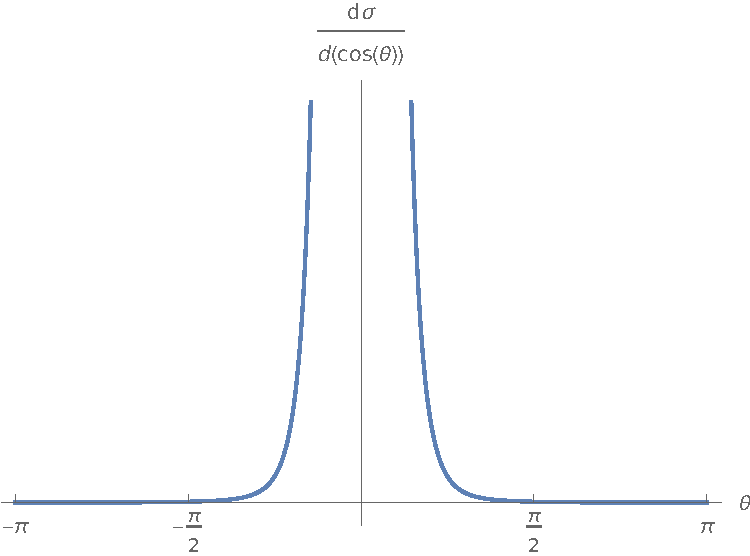
\includegraphics[width=0.4\textwidth]{2}
		\caption{Graph of Eq.~\refeq{ans2} showing divergence as $\tht \to 0$.}
		\label{f2}
	\end{figure}
}






\clearpage
\state{Positronium lifetimes (Peskin \& Schroeder 5.4)}{\hfix}

\prob{
	Compute the amplitude $\cM$ for $\elp \elm$ annihilation into 2 photons in the extreme nonrelativistic limit (i.e., keep only the term proportional to zero powers of the electron and positron 3-momentum).  Use this result, together with our formalism for fermion-antifermion bound states, to compute the rate of annihilation of the $1S$ states of positronium into 2 photons.  You should find that the spin-1 states of positronium do not annihilate into 2 photons, confirming the symmetry argument of Problem~3.8.  For the spin-0 state of positronium, you should find a result proportional to the square of the $1S$ wavefunction at the origin.  Inserting the value of this wavefunction from nonrelativistic quantum mechanics, you should find
	\eq{
		\frac{1}{\tau} = \Gam
		= \frac{\alp^5 \me}{2}
		\approx \SI{8.03e9}{\per\second}.
	}
	A recent measurement gives $\Gam = 7.994 \pm \SI{0.011}{\per\nano\second}$; the 0.5\% discrepancy is accounted for by radiative corrections.
}

\sol{
	The amplitude for $\elp\elm$ annihilation into two photons can be obtained from the Compton amplitude by the substitutions
}


\makebib

\end{document}
